\chapter{黑洞物理}\label{chpt:BH}



\section{Newton 极限与测地线}
尽管这并非真正引力(曲率为零之事实受协变性保护),然而等效赝力所具备的数学形式,将给予我们描述真正引力的灵感。


考虑到生活中的引力场恒稳,物体做匀加速运动。可见在无引力惯性系中研究匀加速运动很有必要,这正是一种比转盘更简单的非惯性运动。

但目前我们只知道 Newton 时空观下匀加速的含义,而在 $\R^{3+1}$ 中呢?这涉及“何种速度对何种时间求导”这样微妙的问题:若认为这种加速度是指相对于某个固定观者的 3-加速,相对论限制告诉我们其不可能一直加速,从而 3-加速必然不能保持恒定,因为在速度较大时它必须减小并趋于零。一种自然的想法是用 4-加速,但为保持正交性,我们至多只能要求其模长恒定。不过 4-加速是时空几何的概念,其时间分量的存在使得任意观者不能直接感知,这是否有意义呢?实际上,代入 $u^i=0$ 于 $A^\mu A_\mu=\gamma^4 a^ia_i+\gamma^6(u^ia_i)^2$ 可知,\textit{质点的 4-加速等于它相对于瞬时静系的 3-加速}。可见,4-加速的意义可在任意情形下,由该观者自己(借助瞬时静系)直接感知,因为 4-加速在此系无时间分量。4-加速模长恒定时,在观者看来这始终是方向和模长上同时恒定的 3-加速。


那么在 $\R^{3+1}$ 中,始终满足瞬时静系 3-加速恒定的质点应走何种轨迹?根据 $A^\mu A_\mu=\gamma^4 a^ia_i+\gamma^6(u^ia_i)^2$ 式,其中在 2 维时空下 $\bm a,\bm v$ 平行,因而 $A^\mu A_\mu=gamma^6 a^2$。考虑到 $\bm A$ 类空性,其模长记为 $A=gamma^3a$ 且恒定。当然,对 $\R^{3+1}$ 而言总可找到一个质点的瞬时静系,因此不妨取一惯性系使质点初速为零。为使始终瞬时静系 3-加速恒定,这样的 4-加速只能同其平行,$A=gamma^3a$ 仍成立。这也说明 $\bm U,\bm A$ 所在平面是固定的,依据对称性可退化至 2 维来研究。我们可根据 $a=\dv*{v}{t},v=\dv*{x}{t}$ 计算曲线 $(t,x)$。设初态 $(0,R)$,一个简单的做法是取

为曲线参数,这样
\[t=\int \frac{\d v}{a}=\int_0^\theta  \frac{\cosh^3\theta}{A}\frac{\d\theta}{\cosh^2\theta}=\frac{\sinh\theta}{A},\]
进而
\[
x=\int v\d{t}=\int_0^\theta \tanh\theta\frac{\cosh\theta\d{\theta}}{A}=\frac{\cosh\theta}{A},
\]
可见轨迹为双曲线 $x^2-t^2=1/A^2$,初态意味着 $A=1/R$。其渐近线相当于原点处的光锥 $C_N$,称为 \textit{Rindler 视界(horizon)}。视界这个名字可理解为界限,从直观上,光信号所传递的信息,不能从光锥另一侧逾越至这边的观者。像这样具有屏障作用的光锥往往暗示着一个视界的存在。可从直觉上做如下类比。在欧氏几何中,一个经历匀速 $v$ 转动的物体(匀速对应正交性),若其加速度模长恒定为 $a$,则轨迹为一圆弧 $x^2+y^2=R^2$,且 $a=v^2/R$。在闵氏几何中,无非是将三角函数替为双曲函数,圆弧也就对应于双曲线。物体在加速度模长恒定时经伪转动走双曲线,且可预料 $x^2-t^2=R^2$ 时 $A^\mu A_\mu=1/R^2$。

\begin{figure}[h!]
    \centering
    \subfloat[\centering 按 $A=1/R$ 均匀分布]{
    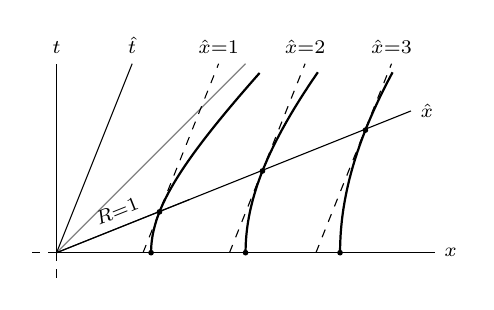
\begin{tikzpicture}[scale=1.2]
    \draw[color=gray] (0,0)--(2,2);
    \draw (0,0)--(4,0) node[right]{$\scriptstyle x$};
    \draw[dashed] (0,0)--(-0.3,0);
    \draw[dashed] (0,0)--(0,-0.3);
    \draw (0,0)--(0,2) node[above]{$\scriptstyle t$};
    \draw (0,0)--({1.3*sinh(0.42)*2.5},{1.3*sinh(0.42)}) node[midway,sloped,above]{$\scriptstyle R=1$};
    \draw (0,0)--(1.5*2.5,1.5) node[right]{$\scriptstyle\hat{x}$};
    \draw (0,0)--(0.8,0.8*2.5) node[above]{$\scriptstyle\hat{t}$};
    \draw[domain=0:1.4,thick,samples=100] plot({cosh(\x)},{sinh(\x)});
    \draw[domain=0:0.85,thick,samples=100] plot({2*cosh(\x)},{2*sinh(\x)});
    \draw[domain=0:0.6,thick,samples=100] plot({3*cosh(\x)},{3*sinh(\x)});
    \foreach \n in {1,2,3}{
    \fill (\n,0) circle(0.03);
    \fill ({\n*cosh(0.42)},{\n*sinh(0.42)}) circle(0.03);
    \draw[dashed] (\n*0.915,0)--(0.8+\n*0.915,0.8*2.5) node[above]{$\scriptstyle\hat{x}=\n$};}
    \end{tikzpicture}
    }
    \quad
    \subfloat[\centering 按 $A$ 相等分布]{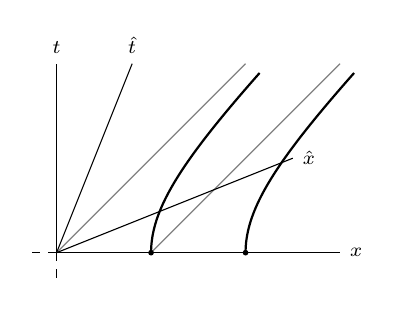
\begin{tikzpicture}[scale=1.2]
    \draw[color=gray] (0,0)--(2,2);
    \draw[color=gray] (1,0)--(3,2);
    \draw (0,0)--(3,0) node[right]{$\scriptstyle x$};
    \draw[dashed] (0,0)--(-0.3,0);
    \draw[dashed] (0,0)--(0,-0.3);
    \draw (0,0)--(0,2) node[above]{$\scriptstyle t$};
    \draw (0,0)--(2.5,1) node[right]{$\scriptstyle\hat{x}$};
    \draw (0,0)--(0.8,0.8*2.5) node[above]{$\scriptstyle\hat{t}$};
    \draw[domain=0:1.4,thick,samples=100] plot({cosh(\x)},{sinh(\x)});
    \draw[domain=0:1.4,thick,samples=100] plot({cosh(\x)+1},{sinh(\x)});
    \fill (1,0) circle(0.03);
    \fill (2,0) circle(0.03);
    \end{tikzpicture}
    }%
    \caption{\small 一系列匀加速观者}
\end{figure}
考虑静置于不戴帽惯性系 $R$ 的 $x$ 轴上的一系列均匀相离的观者,假设它们都沿轴加速运动。如果它们各自的加速度按 $1/R$ 分布,则它们会共用一组 Rindler 视界,因而这些双曲线互相构成伸缩变换。于是易知,若变换至一个具有向右速度的戴帽惯性系 $\hat R$,则在此惯性系看来这些匀加速观者间距未变,且仍然均匀。


然而,若规定各观者加速度一致,则它们各自的双曲线构成平移变换,因而 Rindler 视界也是依次往右排列的。这说明它们不能保持各自间距恒等,因而不同于 Newton 力学的情况。上述讨论说明,按 $A=1/R$ 分布的一系列观者世界线连同一系列 $\hat x$ 轴,可以构成一个新的坐标网格,即其上的点都可用坐标 $(r,\theta)$ 描述,


Newton 引力欲在惯性系中研究引力,这在广相下的含义就是,先用 
 $\eta$  $\mu\nu$ 
 衡量出惯性坐标系,再在此基础上研究弱引力场 
g $\mu\nu$ 
(比如地表引力),其差 
 $\gamma$  $\mu\nu$ =g $\mu\nu$ − $\eta$  $\mu\nu$ 
 在某个惯性坐标系下的 
| $\gamma$  $\mu\nu$ |1。这一近似称为线性引力。此外,在 R
 附近这一点还希望我们关注弱场中的低速运动(无论是试验质点还是场源),这称弱场低速条件,即存在  $\eta$  $\mu\nu$ 
 所衡量的惯性坐标系,使其中所有关心的对象的 3-速率远小于 1。不妨称此系为低速系。Newton 引力学所研究的便是这一类情形,因此又称 Newton 极限。显然可以选择大地系。







为迎合此直觉,我们可将 场直接配置在 $\R^4$ 上,称为 \textit{Schwarzschild 时空}。



\section{黑洞}

广相有三大经典验证,我们将依次介绍。

星光偏折
Eddington(1882-1944,英国天体物理学家) 在 1919 年的一次日食观测中摄下了光线被引力“弯曲”的图片。这一点已经在几何光学近似中从理论上计算过。从那以后,用太阳系的种种检验对场方程作了所谓的\textit{后 Newton 理论(post-Newtonian theory)},这些预测和实验都在这个物理条件下以很高的精度证实了广相.

如果我们考虑黑洞附近的光线,一路走向测地线方程,所描述的轨迹曲线可以作为\textit{引力透镜(gravitational lensing)}的定量解释。

引力红移


假设有一闯入 $r<2M$ 的\textbf{探险者},对其而言,外部空间于其而言仿若永不能逾越的\textit{时间上的过去},而内部空间乃至 $r=0$ 处仿若必将走向的\textit{时间上的未来}。



我们用时空图来理解上述奇性。视界在观感上是一个 3 维空间里的 2 维球面,但在时空图里,它应沿时间方向延伸为一张 3 维类时超曲面。若将时空图绘制为 3 维的,则可以用一个 2 维圆柱面代表视界。若在时空图中标注各点微小光锥的方向,就能将各点时空结构直观地呈现出来,因此欲求出时空中的光线轨迹。光没有质量而走类光线,因此我们不能定义固有时。实际上,描述光线时一般取任意仿射参数 $\lambda$。比如,考虑 $\R^{3+1}$ 中一点 $x_{0}$,此处一个指向未来的类光矢量 $N$ 就可代表光的走向。由 $\alpha(\lambda)=x_{0}+\lambda N$ 定义的直线 $\alpha$ 就是自由光子经过 $x_{0}$ 的世界线。可以预料,上述直线推至一般坐标系甚至一般时空时,应得仿射参数化的测地线方程,对 $\d s^2=0$ 求导很容易证明这一点。实际上,正因为用间隔不变形可得测地线,我们在求某时空的类光测地线时,总是直接处理度规即可,这样便省去克氏符的计算。考虑到球对称性,我们只用 2 个维度
\[
0=\d s^2=-\left(1-{2M}/{r}\right)\,\text d t^2+\left(1-{2M}/{r}\right)^{-1}\text d r^2,
\]
故曲线斜率满足
\[
\left(\dv{t}{r}\right)^2=\frac{1}{(1-2M/r)^2}.
\]
积分得\footnote{严格来讲,$1/x,x\ne 0$ 的不定积分应按定义域分别写出两个可以不同的积分常数,而非直接写 $\ln |x|+C$,但物理学一般偏好用绝对值形式,以尽可能简化研究对象。}
\eq{\label{dia_Sch}
t=\pm\left(r+2M\ln|r-2M|\right)+C.
}
接着要在图中画出上述类光测地线。图上每一点都可确定两条不同的类光测地线,分别属于两\textit{族(family)},因此可均匀地取积分常数以绘制网格。每一条类光测地线都代表光路,因而每一点的光锥面必定切于两族在此处的类光测地线,因此不妨在每个格点都画上一个椭圆,构成一个小“妙脆角”,以代表微小未来光锥(完整光锥用小“沙漏”表示),用以揭示该处的时空结构。所有类光测地线可分为两类。作为未来光锥右侧的称为\textit{外向(outgoing)族},反之为\textit{内向(incoming)族}。比如,注意 $r>2M$ 时,\eqref{dia_Sch} 中正负号取正后斜率为正,只能作为未来光锥右侧,故为外向族。其他情况以此类推。



如图所示,圆柱面为事件视界,波浪线为奇点。可见直接用 Schwarzschild 系使视界出现奇性,生硬地割裂了时空的内外部分。取一个 $r>2M$ 的静态观者,这样由 $\d s^2=-\d\tau^2$ 知其固有时与坐标时的关系\footnote{至此可重新观察 Schwarzschild 度规,若类比钟慢和尺缩效应,我们可将 $1/\sqrt{1-2M/r}$ 理解为 $\gamma$,而这种速度就是 $v=\sqrt{2M/r}$。Newton 理论能给予一个直观理解。物体从引力场某处逃逸的条件是有足够的动能,使得在力场范围内都不为零,这样一旦越过范围就可用剩余动能逃走。最坏的情况是力场范围延至无穷远,则物体动能要足够大,以至于最差只能在无穷远处为零,这样由能量守恒推知速度至少为 $\sqrt{2M/r}$。1799 年,Laplace 假设引力可以吸引光,则对光而言逃脱条件便是 $r>2M$,因此从内部发出的光无法到达无穷远处。这当然不严谨,因为真空光速参考系不变;不能定义光的质量,故光受引力的影响只能由广相解释;内部光线只是无法到达无穷远,仍可超出 $r=2M$ 而至有限远,这与黑洞有本质不同。用 $\gamma$ “推导”引力度规的方式可见文献 Czerniawski。}为
\eq{
\d\tau=\sqrt{1-2M/r}\d{t},
}
这说明,静态观者借自己的标准钟观察一个探险者,会发现其落入 $r=2M$ 的过程逐渐缓慢,因为
\[
\dv{t}{\tau}=\frac{1}{\sqrt{1-2M/r}}
\]
会从 1 逐渐递增至 $r=2M$ 处发散,进而其在 $r=2M$ 附近“毫无动静”,仿佛时间停滞流逝,最终将永远定格于 $r=2M$ 而不会坠入视界。然而在探险者看来,他进入视界“确实”是顺理成章的。$r>2M$ 的部分让人误解为任何质点永远位于视界之外,因为我们容易把 $t\to\infty$ 混同于“永远”。古希腊时期有一著名的 Zeno 悖论讨论过类似效应。Zeno 为讨论无穷的含义设计了这样的情形:一位运动员 Achilles 欲同一只乌龟(tortoise)赛跑,且乌龟起点先于他若干路程 $L$。按常理来说,他的速度 $v_1$ 快于乌龟的 $v_2$,明显会在有限时间 $L/(v_1-v_2)$ 内超过乌龟。但设想这样计时:他欲超过乌龟,必须先追至乌龟的起点,但一旦如此,乌龟又能前进若干步,这样便有新的起点等着他,如此这般有无穷多这样的起点,则他“永远”也赶不上乌龟。实际上这并不存在孰是孰非的问题,因为答案是相对于所选取的计时方式而言的。乌龟均匀向前,它未“想得”那么复杂,因此可将“乌龟时”理解为和观众一致认同的普通时 $t$。Achilles 时(或称 Zeno 时) 记作 $t'$,两种时间皆起于零。当 $t=L/v_1$ 时,Achilles 到达乌龟在 $t'=0$ 时的起点,则 $t'$ 加一,以此类推有
\[
t=\sum_{i=0}^{t'-1} \frac{L}{v_1}\left(\frac{v_2}{v_1}\right)^{i}=\frac{L}{v_1-v_2}\bigg(1-\bigg(\frac{v_2}{v_1}\bigg)^{t'}\bigg),
\]
上式自然将 $t'$ 从 $\N$ 延拓至 $\R_+$,因此从 Achilles 时 $t$ 到乌龟时 $t'$ 的变换为
\[
t'=\frac{1}{\ln(v_2/v_1)}\ln\left(1-\frac{v_2-v_1}{L}t\right),
\]
可见二者走势一致,区别在于 $t'$ 会在 $t=L/(v_2-v_1)$ 发散。



这给了我们寻找新坐标的启发。我们亦可给视界赋予发散的坐标,这样就可将度规的奇性隐藏在坐标变换中。先想办法消除度规中的因子 $(1-2M/r)^{-1}$。常常采取因式分解,即
\[
\d s^2=\left(1-{2M}/{r}\right)\left(-\d t^2+\left(1-{2M}/{r}\right)^{-2}\d r^2\right),
\]
定义一个新半径使得
\eq{
\d r_*=\frac{\d r}{1-2M/r}\Rightarrow r_*=r+2M\ln\abs{\frac{r}{2M}-1},
}
这里取积分常数使得 $r=0$ 时 $r_*=0$,可见其与 $r$ 走势一致而仅在 $r=2M$ 处发散。类比 Zeno 悖论,可称\textit{乌龟坐标}。度规就可表为
\[
\d s^2=(1-2M/r)\left(-\d t^2+\d r_*^2\right),
\]
这样就消除了发散因子。然而这个变换并不够,因为其行列式 $g$ 在 $r=2M$ 为零,意味着逆矩阵元发散。但是这种变换很常用,值得单独命名并继续使用。对物理量 $x$,变换 $x'=x+(r_*-r)$ 在 $r<2M$ 时 $x'<x$,故称\textit{超前(advanced)变换},而 $x'=x-(r_*-r)$在 $r<2M$ 时 $x'>x$,故称\textit{推迟(retarded)变换}。考虑到奇性导致了类似于 Zeno 悖论的现象,应将坐标时 $t$ 超前变换至 $\tilde t$,则度规表为
\eq{
\d s^2=-\left(1-\frac{2 M}{r}\right) {\d \tilde t}^2+\frac{4M}{r}\,\mathrm{d} \tilde t\, \mathrm{d} r+\left(1+\frac{2 M}{r}\right)\d r^2,
}
便可使时空交叉项为正,符合黑洞演化的方向。上式在 $r=2M$ 处所有分量皆收敛,而行列式 $g=-(g_{01})^2\ne 0$,这才算消去奇性。该坐标系称为\textit{超前 Eddington 系}。利用十字相乘法可分解出两个类光测地线族,其一是
\eq{
\dv{\tilde t}{r}=\frac{r+2M}{r-2M}\Rightarrow \tilde t=r+4M\ln\abs{r-2M}+C_1, \quad r=2M,
}
其二是
\eq{
\dv{\tilde t}{r}=-1\Rightarrow \tilde t=-r+C_2.
}
显然前者为外向族而后者为内向族。进而可画得图 \ref{fig:mink}。
\begin{figure}[h!]
    \centering
    \includegraphics[width=.6\textwidth]{fig/chpt02/schBH.pdf}
    \caption{静态黑洞时空图}
    \label{fig:mink}
\end{figure}
其中设有一个静态观者和一个位于 $\tilde t$-$r$ 平面的探险者。可见视界外的质点可以穿越视界进入黑洞,而一旦进入就无法逃逸,并最终落入奇点。探险者若想摆脱黑洞的引力束缚,只能采用某种喷气火箭,以大于该处静态观者所需力量向右飞行。一旦燃料储备不足,便连静态观者也当不了。假设其燃料充足,若探险者企图接近视界而迅速掉头离开,则越近风险越大,因为从 $r=2M$ 附近逃离须使飞船接近光速。并且,当视界内部很空旷时,对探险者而言,其进入视界时并无触觉,若稍有不慎,未能警觉自己所处位置,则很可能多走一步而遁入厄运。当然,探险者还是能通过视觉上“眼前一黑”来观察,但更可怕的是,探险者并非真正的质点,而不同位置所受引力在此极端地带将差距巨大,因此潮汐力(对应于曲率大小)极有可能撕碎探险者,除非视界半径很大而稀释了曲率。此外,前文用测量效应说明了静态观者对探险者的观察,亦可用视觉效应这种现象。若静态观者借光信号观察探险者,则从图 \ref{fig:mink} 容易看出,随探险者逐渐接近视界,探险者所发出的光将越来越晚地到达静态观者,而坠入的画面无法传播出来。

能描述 Schwarzschild 时空的坐标系有很多,超前 Eddington 系并非完美无缺。比如,Schwarzschild 系能保证 $g_{01}=0$ 而超前 Eddington 系不然。可能存在一个“更好”的坐标系既能消除奇性,又能使 $g_{01}=0$。第 

节就提过研究弯曲时空引力性质的技巧,那就是到平直时空的加速度系去,而 Rindler 坐标系正好能满足 $g_{01}=0$,我们可从中获取灵感。考虑到 Rindler 系的坐标具备时空的性质(尤其是远处的加速系),现在就将其改记 $(t,x)$。不妨先讨论 $x>0$,反之情形同理。原来的闵氏系改记 $(T,X)$。这样闵氏度规 $\d s^2=-\d T^2+\d X^2$ 在坐标变换 $X=x\cosh t,T=x\sinh t$ 下变为“Rindler 度规” $\d s^2=-x^2\d t^2+\d x^2$,二者无实质区别,为同一度规。现在我们不再按 $T,X$ 正交来绘制时空图,而是按 $t,x$ 正交。再次声明,读者无需感到诧异,同一时空由于所用坐标系不同,时空图可千差万别。同理求出内、外向族分别为
\[
t=-\ln x+C_1,\quad t=\ln x+C_2.
\]
故可绘制如下图 。注意,闵氏度规在 Rindler 系是有奇性的,因为其行列式 $g=-x^2$ 在 $x=0$ 处为零。可见,Rindler 系和闵氏系的相对地位,就像是 Schwarzschild 系或 Eddington 系和“更好”坐标系的相对地位。


类光测地线意味着 $\d s^2=0$,而张量为零的事实不受坐标系影响,因此上述类光测地线族其实“对应于”闵氏时空里的类光测地线族
\[
T=-X+C_1,\quad T=X+C_2.
\]
第  节中将双曲线、射线视作坐标线而衍生出 Rindler 坐标系,仿照这一思想,欲视类光测地线族为坐标网格(称为\textit{类光坐标})。在 Rindler 图  里,这是在令
\eq{
v=t+\ln x,\quad u=t-\ln x.
}
度规表为 $\d s^2=-\e^{v-u}\d v\d u$。而在闵氏图里是令
\eq{
V=T+X,\quad U=T-X,
}
或
\eq{
T=\frac{V+U}{2},\quad X=\frac{V-U}{2},
}
这有双曲函数的形式,而 $T,X$ 与 $t,x$ 的变换正是双曲函数,故易知如下指数式
\eq{
V=\e^v>0,\quad U=-\e^{-u}<0.
}
度规现表为 $\d s^2=-\d V\d U$,不存在任何坐标奇性。
\begin{figure}[h!]
    \centering
    \includegraphics[width=.6\textwidth]{fig/chpt02/rindler.pdf}
    \caption{消除 Rindler 系的坐标奇性}
    \label{fig:rindlerIM}
\end{figure}
如图 \ref{fig:rindlerIM} 所示,则从直观上,闵氏时空图就像是把 Rindler 图 里竖直的 $x=0$ 从 $t=0$ 处向右“掰弯”成如光锥面一般的 Rindler 视界 $T^2=X^2$,即 $VU=0$,由上式知 $V,U$ 轴正方向如图 \ref{fig:rindlerIM}。图中蓝色双曲线代表等 $r$ 线,红色射线代表等 $t$ 线。可见,从 Rindler 图到闵氏图经历了如下过程:
\[
(t,x)\to(v,u)\to(V,U)\to(T,X).
\]
依葫芦画瓢地寻找“更好”坐标系。在超前 Eddington 系中,时间对角项在 $r=2M$ 为零,为消除奇性,只能借由超前变换所产生的非零时空交叉项,但我们并不想要交叉项。可见,必须使 $T,X$ 坐标的时间对角项非零。回到 Schwarzschild 系。不妨先研究 $r>2M$。$v,u$ 从类光测地线族产生,注意式 \eqref{dia_Sch} 与 $t=\pm r_*$ 相差常数,因此内、外向族分别给出
\eq{
v=t+r_*,\quad u=t-r_*.
}
由于 $r_*$ 作了超前变换,因此前者称\textit{超前类光坐标},后者称\textit{推迟类光坐标}。可见对 Rindler 时空来说其乌龟坐标是 $x_*=\ln x$,读者很容易验证这一点。度规在 $v,u$ 下表为
\[
\d s^2=-(1-2M/r)\d v\d u,
\]
沿用 $V,U$ 的指数形式但预留待定常数(只可与 $M$ 有关)以使最终的时间对角项非零\footnote{有种做法是填上 $1/\beta=4M$ 因子以约去指数求导出的系数,这样度规 \eqref{eq:kruskal} 中 ${32M^3}/{r}$ 变为 $2M/r$。}:
\eq{
V=\e^{\beta v}>0,\quad U=-\e^{-\beta u}<0.
}
只预留一个是考虑到对称性。进而度规表为
\[
\d s^2=-\beta^{-2} (1-2M/r) \e^{\beta(u-v)} \d V\d U,
\]
考虑到 $T,X$ 系只是 $V,U$ 系的旋转,我们可将其定义沿用至此,则 $-\d V\d U=-\d T^2+\d X^2$,进而保证无交叉项。现在的目标就是约掉 $(1-2M/r)$ 通分后所含因子 $(r-2M)$。这份任务只能交由 $\e^{\beta(u-v)}$,我们就要用 $r$ 表示它(由稳态条件可预料无 $t$)。注意 $u-v=-2r_*$,代入 $r_*$ 定义有
\[
\e^{\beta(u-v)}=\e^{-2\beta r}\left(\frac{2M}{r-2M}\right)^{4\beta M},
\]
说明应取 $\beta=1/4M$,则
\[
\d s^2=-\frac{32M^3}{r}\e^{-r/2M}\d V\d U=\frac{32M^3}{r}\e^{-r/2M}(-\d T^2+\d X^2).
\]
这里仍留有一个不能消除的时空奇点 $r=0$,与 Rindler 情况有所不同。综上,还原另外两个空间维度后,Schwarzschild 度规就表为
\eq{\label{eq:kruskal}
\d s^2=\frac{32M^3}{r}\e^{-r/2M}(-\d T^2+\d X^2)+r^2\d\Omega^2,
}
这里 $r$ 视作 $T,X$ 的函数,易知
\eq{
X^2-T^2=-VU=\e^{(v-u)/4M}=\left(\frac{r}{2M}-1\right)\e^{r/2M},
}
注意 $r>0$,我们可用数学中的 \textit{Lambert 函数}
\eq{
y=\operatorname{W}(x)\Longleftrightarrow x=y\e^y,y\geqslant -1
}
将其表为
\eq{\label{eq:r=T,X}
r=2M\operatorname{W}\left(\frac{X^2-T^2}{\e}\right)+2M.
}
这个坐标系称为 \textit{Kruskal 系}。我们再次按 $T,X$ 正交绘制 2 维时空图。$(-\d T^2+\d X^2)$ 形式的保留使类光测地线斜率仍为 $\pm 1$。实际上,像这样给原度规乘以一个正因子就称为 \textit{Weyl 重标度(rescaling)变换},简称 Weyl 变换,它能保留时空结构,故又称为\textit{共形(conformal)变换}。
\begin{figure}[h!]
    \centering
    \includegraphics[width=.6\textwidth]{fig/chpt02/kruskal.pdf}
    \caption{Kruskal 延拓}
    \label{fig:kruskal}
\end{figure}
从图 \ref{fig:kruskal} 上可见,Kruskal 系也会“掰弯” Schwarzschild 时空的视界 $r=2M$,使之变为光锥面 $VU=0$。易知各坐标的取值分布同图 \ref{fig:rindlerIM} 相似。然而,我们只考虑了 $r>2M$ 的情况,在图上标记为开区域 \textit{A 区},对应 $V>0,U<0$。那 $r<2M$ 呢?Schwarzschild 系的 $r>2M$ 和 $r<2M$ 借超前 Eddington 系消除 $r=2M$ 坐标奇性。
从图上看,从 A 区任意点出发的内向类光线一定坠向 $V$ 正半轴,说明其代表事件视界,故可记作 $\H_V^+$。Kruskal 系也能消除坐标奇性,我们可越过视界来到上方,这里 $V,U>0$,说明我们自然地拓宽了 $V,U$ 的定义。为使 $U$ 为正,应定义
\eq{
V=\e^{v/4M}>0,\quad U=\e^{-u/4M}>0,
}
可验证度规仍表为 \eqref{eq:kruskal} 式。这里等 $r$ 线应无限延伸,因为等 $t$ 线从 $U$ 正半轴至 $V$ 正半轴遍历了所有 $t$ 值。一系列等 $r$ 线至多扫至时空奇点 $r=0\Leftrightarrow T^2-X^2=1$ 而无法越过,所扫区域里的任意类时、类光线确实都坠入奇点,说明其代表黑洞,称为 \textit{B 区}。可见,超前 Eddington 系覆盖了 $\mathrm{A}\cup\H_V^+\cup\mathrm{B}$,即整个 Schwarzschild 时空。奇点及其外部红色区域不属于时空。综上,A,B 区的坐标变换可整合为
\eq{
V=\e^{(r_*+t)/4M},\quad U=-\sgn(r-2M)\e^{(r_*-t)/4M}.
}
进而变换至 $T,X$ 可整合为
\eq{\begin{aligned}
    T&=\frac{\e^{r/4M}}{2}\sqrt{\abs{\frac{r}{2M}-1}} \left(\e^{t/4M}-\sgn(r-2M)\e^{t/4M}\right),\\
    X&=\frac{\e^{r/4M}}{2}\sqrt{\abs{\frac{r}{2M}-1}} \left(\e^{t/4M}+\sgn(r-2M)\e^{t/4M}\right).
\end{aligned}}
其仍形如双曲函数。若从 $T,X$ 做逆变换,易知 $r$ 仍满足 \eqref{eq:r=T,X} 式,而 $t$ 表为
\eq{
t=2M\ln\frac{X+T}{|X-T|},
}
形如反双曲正切函数。


\section{引力坍缩}\label{sec:collapse}

星体演化

这些问题花了很长时间才理清,因为整体微分几何的流形语言是在场方程之后才发展完整的。

人们现在普遍认为星体\textit{引力坍缩(gravitational collapse)}的末日归宿就是黑洞。

进入黑洞的测地线会在有限固有时内碰上奇点而“断掉”,不可无限制地延伸下去,称作\textit{不可延测地线(inextendible geodesic)}。接近奇点的宏观观者会被差距强烈的潮汐力撕碎。

这种病态性质与高度的球对称性有关。Penrose 在 1965 年给出的\textit{奇性定理(singularity theorem)}中指出,耦合适当的物质并附加某些条件后,一定会出现不可延测地线,因而就产生了这么个奇点。奇性定理给出了两个重要猜想(conjecture)或者假设(hypothesis)。第一个是\textit{弱宇宙监督(weak cosmic censorship)假设}: 对于适当的物质方程组和一般物理意义的初始条件,奇点一定限制在黑洞区域内而“看不见”; 第二个是\textit{强(strong)宇宙监督假设}:解的奇性一定与其延拓遇到局部阻碍有关。后一个假设保证了动力学问题的唯一解必定是初始数据产生的经典时空,即\textit{经典决定性原理(Classical Newtonian determinism)}。如果抛弃条件的一般性,则这两个假设都不成立。Christodoulou 做出过标量场方程组的球对称解,其中的奇点就不在黑洞区域内,这样的时空就称作包含了\textit{裸(naked)奇点}。裸奇点很容易构造出来,比如直接令 $m<0$,但此时就不允许\textit{渐近平直(asymptotically flat)的 Cauchy 面}了,因而可能不太符合咱们的物理常识。这件事与所谓的\textit{正能量定理(positive mass theorem)}有关.


\section{Penrose 图}

\section{时空延拓}

\section{嵌入图与虫洞}
绘制虫洞的一个形象方法就是用嵌入图。


\section{RN 黑洞}



\section{黑洞热力学}

KN 黑洞

黑洞无毛猜想

\section{dS 与 AdS 时空}\label{sec:dS}



\section{轴对称时空}
    \subsection{Kerr 度规}
    \subsection{KN 度规}

\section{黑洞热力学}
\subsection{孤立视界}
\subsection{类光 Raychaudhuri 方程}
\subsection{信息论}


后 Newton 力学
